\documentclass [bachelor,german,a4paper,11pt,oneside,webreferences,glossary,indextop,listoflistings,listofalgorithms]{INSOthesis}
% change encoding in the document
%\inputencoding{utf8} % default
%\inputencoding{latin1} % for windows

\thesistitle{Evaluierung von REST Frameworks für Android im Kontext des Revex2020 Projekts}
\thesisshorttitle{Evaluierung von REST Frameworks}
%\thesissubtitle{Optional Subtitle} % optional
\thesisdate{\today}

% all titles and designations have to be gender-related!
%\thesistype{Diplomarbeit}{Master's Thesis}
%\thesisdegree{Diplom-Ingenieurin}{Diplom-Ingenieurin}
\thesiscurriculum{Software Engineering and Internet Computing}{Software Engineering and Internet Computing} % your study
\thesisauthor{Elisabeth Pilz} % your name
\thesisauthoraddress{Luegstraße 13, 3340 Waidhofen Ybbs} % your address
\thesismatrikelno{1225231} % your registration number

% advisor
%\thesisauthorpreamble {Verfasser}
%\thesisadvisorpreamble {Betreuung}
%\thesisadvisorone {Thomas Grechenig}
\thesisadvisortwo {Dominik Moser}
%\thesisadvisorthree {Vorname Nachname}

% Bibliographie file
\bibliography{bibliography/references}

\hypersetup{
  %colorlinks=false % enable and disable frames arround links
}

%%%%%%%%%%%%%%%%%%%%%%%%%%%%%%%%%%%%%%%%%%%%%
%
% Can be used to add additional informations
%
%%%%%%%%%%%%%%%%%%%%%%%%%%%%%%%%%%%%%%%%%%%%%
% \AfterTitlePages{}
% \AfterDeclaration{}
% \AfterAcknowledgements{}
% \AfterAbstract{}
% \AfterListOfFigures{}
% \AfterListOfTables{}
% \AfterAbbreviations{}
% \AfterBibliography{}

\renewcommand\afterchapternum{\hspace{1em}}
\begin{document}

\maketitle

%%%%%%%%%%%%%%%%%%%%%%%%%%%%%%%%%%%%%%%%%
%%%   CONTENTS    %%%%%%%%%%%%%%%%%%%%%%%
%%%%%%%%%%%%%%%%%%%%%%%%%%%%%%%%%%%%%%%%%

%%%%%%%%%%%%%%%%%%%%%%%%%%%%%%%%%%%%%%%%%%%%%%%%%%%%%%%%%%%%%%%%%%%%%%%%
\chapter{Einleitung}
\label{sec:introduction}
%%%%%%%%%%%%%%%%%%%%%%%%%%%%%%%%%%%%%%%%%%%%%%%%%%%%%%%%%%%%%%%%%%%%%%%%

%=======================================================================
\section{Problemstellung}
%=======================================================================
Einer der größten Trends auf den Business-Markt ist die Mobilisierung der Geschäftswelt, die sich in den verschiedensten Unternehmensstrategien widerspiegelt. Es gibt zahlreiche Innovationen, um unabhängig von Stakeholdern, Zeit, Ort und Geräten auf Daten und Anwendungen zuzugreifen. Ein wesentlicher Innovationsstrang ist dabei die Entwicklung von Business-Apps, um beispielsweise die Arbeitszeiten auf Geschäftsreisen effektiv ausnützen zu können. Dadurch hat die Bedeutung der Informations- und Kommunikationsindustrie in den letzten Jahren in den Unternehmen stetig zugenommen \cite{smartMobileApps1}.
\\\\
Durch die immer stärkere Nachfrage nach mobilen Apps im Arbeitsalltag ist es notwendig, mobile Endgräte in bestehende Geschäftsprozesse der Unternehmen zu integrieren. Dabei soll es vermieden werden, eine komplett neue IT-Infrastruktur unter Beteiligung von mobilen Endgeräten zu schaffen. In vielen Unternehmen wird daher die IT-Anwendungslandschaft an das Paradigma der serviceorientierten Architektur ausgerichtet. Ein wesentlicher Vorteil dabei ist, dass wohl definierte Schnittstellen vorhanden sind und angebotene Dienste flexibel und plattformunabhängig genutzt werden können. Sollen nur mobile Anwendungen in die existierende IT-Anwendungslandschaft eingegliedert werden, bedeutet dies in der serviceorientierten Architektur, das Web Services benötigt werden. In der Praxis werden Web Services entweder mit dem Kommunikationsprotokoll \acrfull{SOAP} oder \acrfull{REST} umgesetzt \cite{smartMobileApps17}.
\\\\
Im Revex2020 Projekt wird das Kommunikationsprotokoll REST verwendet, dadurch ist es nötig ein geeignetes Framework aufseiten der mobilen App zu finden, dass eine vollständige und korrekte Anbindung an den Webservice ermöglicht. Es existieren bereits zahlreiche Frameworks, die eine REST Implementierung unterstützen, diese unterscheiden sich aber stark in der Qualität und im Funktionsumfang. Auch bieten nicht alle diese Frameworks eine Unterstützung für Android an. Daher ist die Auswahl eines geeigneten Frameworks für eine erfolgreiche Implementierung ausschlaggebend. 

%=======================================================================
\section{Motivation}
%=======================================================================

Die Thematik rund um REST-Frameworks für Android ist noch relativ neu, dadurch ist es nicht möglich ohne größere Recherchen ein geeignetes Framework für das Projekt Revex2020 auszuwählen. Es gibt zwar einige Vergleiche von REST Frameworks, wie etwa die Fachstudie von Markus Fischer, Kalman Kepes und Alexander Wassiljew \cite{vergleich13}. In dieser Studie wird allerdings nicht darauf eingegangen, ob die Frameworks eine Implementierung clientseitig mit Android unterstützen, es wird die vermehrt auf die serverseitige Implementierung eingegangen. Die Möglichkeit der clientseitigen Implementierung ist aber eine essenzielle Anforderung, da eine Business-App für Android entwickelt werden soll. 
\\\\
Der immer stärker wachsende Bereich von mobilen Anwendungen macht das zu untersuchende Thema besonders interessant. Herkömmliche Software rückt immer weiter in den Hintergrund, Daten sollen sofort und überall abgerufen werden können. Mobile Endgeräte wie Smartphone und Tablets verändern daher die Geschäftswelt nachhaltig, Führungskräfte und Mitarbeiter erhalten jederzeit Zugang zu Unternehmensinformationen und -prozessen. Die Unternehmen der Zukunft werden daher mobil \cite{smartMobileApps7}.  
\\\\
Revex2020 ist ein Forschungsprojekt zur Revitalisierung von Wasserkraftwerken, das in Kooperation mit dem Institut für Energietechnik und Thermodynamik entwickelt wird \cite{doujak}. Ein Ziel dieses Projektes ist es, Mitarbeitern zukünftig zu ermöglichen, mithilfe von mobilen Endgeräten den Zustand einzelner Kraftwerkskomponenten vor Ort erfassen zu können. Es soll eine Android-App entwickelt werden, die das bereits vorhandene Backend, über das REST-Webservices nutzt um exemplarisch den Anwendungsfall abzubilden.

%=======================================================================
\section{Zielsetzung}
%=======================================================================

Ziel dieser Bachelorarbeit ist die Evaluierung verschiedener REST-Frameworks für Android im Kontext des Revex2020 Projekts, um eine unkomplizierte Anbindung an das bereits vorhandene Backend zu ermöglichen. Dazu werden bestehende REST-Frameworks für Android getestet, indem diese in einem Anwendungsfall eingesetzt werden. Nach der Evaluierung dieser Frameworks soll eine Empfehlung abgegeben werden, welches sich am besten für das Revex2020 Projekt eignet.
\\\\
Die Evaluierung der Frameworks erfolgt anhand von Prototypen, indem die REST-Frameworks verwendet werden. Es wurden im Vorfeld verschiedene Anwendungsfälle definiert (siehe Abbildung \ref{figure:useCase}), indem die einzelnen REST Frameworks integriert werden. Dabei werden in einem Szenario verschiedene Prozesse durchgespielt, wie Kraftwerk erstellen, löschen, bearbeiten und anzeigen. Als Vorlage dazu wurde die bestehende Web-Applikation des Projektes verwendet.
\\\\

\begin{minipage}{\textwidth} 
	\centering	
	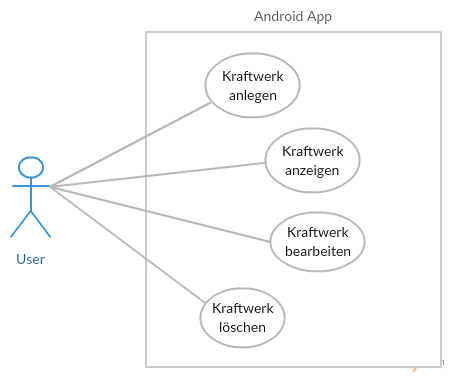
\includegraphics[width=0.65\textwidth]{figures/kraftwerke_use_case.png}
	\captionof{figure}{Use-Case-Diagramm}
	\label{figure:useCase}
	\vspace{2ex}
\end{minipage}

%=======================================================================
\section{Methodik}
\label{sec:methodik}
%=======================================================================
Die Qualität der einzelnen Frameworks soll anhand folgender Kriterien verglichen werden, welche an dem Kriterienkatalog der Fachstudie "Vergleich von Frameworks zur Implementierung von REST-basierten Anwendungen" \cite{vergleich13} angelehnt sind. Dieser Kriterienkatalog beschäftigt sich mit den Eigenschaften für die Evaluierung von REST Frameworks, vor allem auf serverseitiger Sicht. Der Kriterienkatalog wurde deshalb gekürzt bzw. einzelne Punkte zusammengefasst und abgeändert, um eine Evaluierung im Kontext des Projektes Revex2020 durchführen zu können. 
\\\\
Das Hauptaugenmerk der Evaluierung liegt auf der Clientseite, da die entwickelte App eine Client Applikation darstellt. Deswegen wurden spezifische Kriterien der Fachstudie zu einer REST Server Applikation gestrichen. Beispielsweise wurde der gesamte Kriterienblock über Ressourcentypen \cite{ressourcen:rest} weggelassen, da es für die clientseitige Verarbeitung irrelevant ist, welche Ressourcentypen serverseitig implementiert werden können. 
\\\\
\textbf{Entwicklungskultur rund um die Frameworks:}
\begin{itemize}
	\item Unter welcher Lizenz steht das Projekt zur Verfügung?
	\item Existiert eine aktive Community?
	\item Ist eine Dokumentation des Codes vorhanden? (Schnittstellenbeschreibung, JavaDoc)	
	\item Gibt es Hilfestellung für Entwicklung? (Tutorial, Codebeispiele)
\end{itemize}

\textbf{Implementierung der REST-Frameworks:}
\begin{itemize}
	\item Wie aufwendig ist es das Framework ins Projekt einzubinden? 
	\item Welche HTTP-Methoden werden unterstützt? (GET, POST, PUT, DELETE etc.)
	\item Gibt es Möglichkeiten den HTTP-Header zu verändern oder zu erweitern?
	\item Welche Medientypen werden unterstützt? (JSON, HTML, XML etc.)
	\item Kann die URL zum Abfragen von Resourcen dynamisch verändert werden? (z.B. über Parameter steuern)
	\item Gibt es eine Möglichkeit für asynchronen Nachrichtenaustausch?
	\item Wird das HATEOAS-Konzept* unterstützt?
	\item Wird ein Error-Handling unterstützt?	
\end{itemize}

\textbf{Performance und benötige Speicherplatz der Frameworks:}
\begin{itemize}
	\item Wie stark wird die CPU belastet?  
	\item Wie viel RAM wird benötigt? 
	\item Wie schnell erfolgt die Abwicklung einzelner Requests (GET, POST)?
	\item Wie groß ist die erzeugte .apk-Datei?	
\end{itemize}
\newpage
\textbf{Erweiterte Technische Fähigkeiten der Frameworks:}
\begin{itemize}
	\item Wie wird Sicherheit gehandhabt?  (Authentifizierung)
	\item Werden andere Protokolle fernab von HTTP unterstützt?	
	\item Unterstützt das Framework die Entwicklung von Server Applikationen?
	\item Bietet das Framework zusätzliche Dienst fernab der REST-Kommunikation an?
	\item Wird transaktionales Verhalten vom Framework unterstützt? (ACID**-Eigenschaften)\\
\end{itemize}

* Das \textbf{HATEOAS}-Konzept wird in Kapitel \ref{sec:rest} genauer beschrieben.
\\\\
** \textbf{ACID} seht für Atomicity, Consistency, Isolation und Durability. Dieses Konzept beschreibt, dass alle Daten die während einer Transaktion verwendet werden, gesperrt sind und sich nicht ändern dürfen, so lange bis die Transaktion Commited wird oder ein Rollback durchgeführt wird. Das Einhalten dieser Eigenschaften ist wichtig, da die Kommunikation zu Servern über zustandslose REST-Schnittstellen abgewickelt wird. Durch die Zustandslosigkeit der Anfragen kann es bei Fehlern schnell zu einer Dateninkonsistenz auf dem Server kommen \cite{braun:Transaktionen}.

%%%%%%%%%%%%%%%%%%%%%%%%%%%%%%%%%%%%%%%%%%%%%%%%%%%%%%%%%%%%%%%%%%%%%%%%
\chapter{Grundlagen}
\label{sec:fundamentals}
%%%%%%%%%%%%%%%%%%%%%%%%%%%%%%%%%%%%%%%%%%%%%%%%%%%%%%%%%%%%%%%%%%%%%%%%

In diesem Kapitel werden die theoretischen Grundlagen und alle in der Arbeit verwendeten und für das Verständnis relevante Begriffe erläutert. Kapitelnamen spezifizieren, anpassen an die Fragestellung der Arbeit.

\makeatletter\ifthesis@masterthesis
Nach dem Lesen dieses Kapitels sollten folgende Punkte klar dargestellt sein:
\begin{itemize}
	\item Beschreibung der relevanten theoretischen Grundlagen für die Behandlung der Fragestellung
	\item Detaillierte Beschreibung ggf. vorhandener relevanter Spezifika des Anwendungsbereichs, in dem das Problem gelöst wird
	\item Detaillierte Beschreibung relevanter Spezifika eingesetzter Technologien
	\item Analyse bestehender Ansätze/ Vorarbeiten: Literaturstudium, Analyse, Vergleich und Zusammenfassung bestehender Ansätze.
\end{itemize}
\fi\makeatother

Gerade im Bereich der Grundlagen wird viel Literatur zitiert -- Details zum Zitieren finden Sie im Kapitel \ref{sec:references}. Da keine Diplomarbeit so innovativ ist, dass sie nicht auf vorhandenes Wissen aufbaut und in ein entsprechendes Forschungsumfeld eingebettet ist, kommt an dieser Stelle der Literaturrecherche eine besondere Bedeutung zu. Als Daumenregel gilt, dass der aktuelle Stand der Wissenschaft in der Informatik üblicherweise durch Publikationen v.a. der letzten 2 – 4 Jahre repräsentiert wird.

\makeatletter\ifthesis@masterthesis
Beispielhaft einleitender Text an dieser Stelle:\\
Dieses Kapitel stellt Konzepte der Informationstheorie vor und liefert theoretische Grundlagen zu verdeckten Kanälen. Die verdeckte Kommunikation wird mit den verwandten Techniken der Steganographie und Kryptographie verglichen. Außerdem werden ein einfaches Fehlerkorrekturverfahren sowie die Grundlagen des HTTP-Protokolls beschrieben.
\fi\makeatother

%=======================================================================
\section{Aktueller Stand der Technik}
%=======================================================================

In diesem Kapitel wird ein Überblick über bereits existierende Lösungen für die Problemstellung bzw. verwandte Problemstellungen gegeben. Dabei ist eine Klassifizierung der existierenden Lösungen empfehlenswert. Eine Analyse der Lösungen, nach Kriterien sortiert, sollte insbesondere auch die Defizite der existierenden Lösungen erläutern und damit insbesondere auch eine Begründung liefern, warum diese Lösungen für die Problemstellung der Arbeit nicht herangezogen werden können.

%-----------------------------------------------------------------------
\subsection{Unterkapitel}
%-----------------------------------------------------------------------

Bei der Verwendung von Gliederungsebenen gibt es Folgendes zu beachten:
\begin{itemize}
	\item Es sollten nicht mehr als 3 Gliederungstiefen nummeriert werden.
	\item Unterkapitel sind nur dann sinnvoll, wenn es auch mehrere Untergliederungen gibt. Ein Kapitel 2.1.1 sollte somit nur dann verwendet werden, wenn es auch 2.1.2 gibt.
	\item Oft ist es einfacher und besser verständlich, Aufzählungen als Text zu formulieren und somit weitere Gliederungsstufen zu vermeiden.
\end{itemize}

%-----------------------------------------------------------------------
\subsection{Abbildungen}
\label{sec:abbildungen}
%-----------------------------------------------------------------------

Beschreibungen zu Abbildungen und Tabellen stehen unter dem Bild. Jede Abbildung muss im Fließtext referenziert werden. In \LaTeX besitzen Abbildungen typischerweise Labels, welche zum referenzieren verwendet werden. Zudem plaziert \LaTeX die Abbildungen an geeigneten Stellen, was meistens auch wünschenswert ist. Falls das nicht gewünscht wird, kann es durch Optionen beeinflusst werden.

Abbildung \ref{fig:xxx} verdeutlicht  \dots\\
(siehe Abbildung \verb|\ref{<label>}|)

\begin{figure}
	\centering
	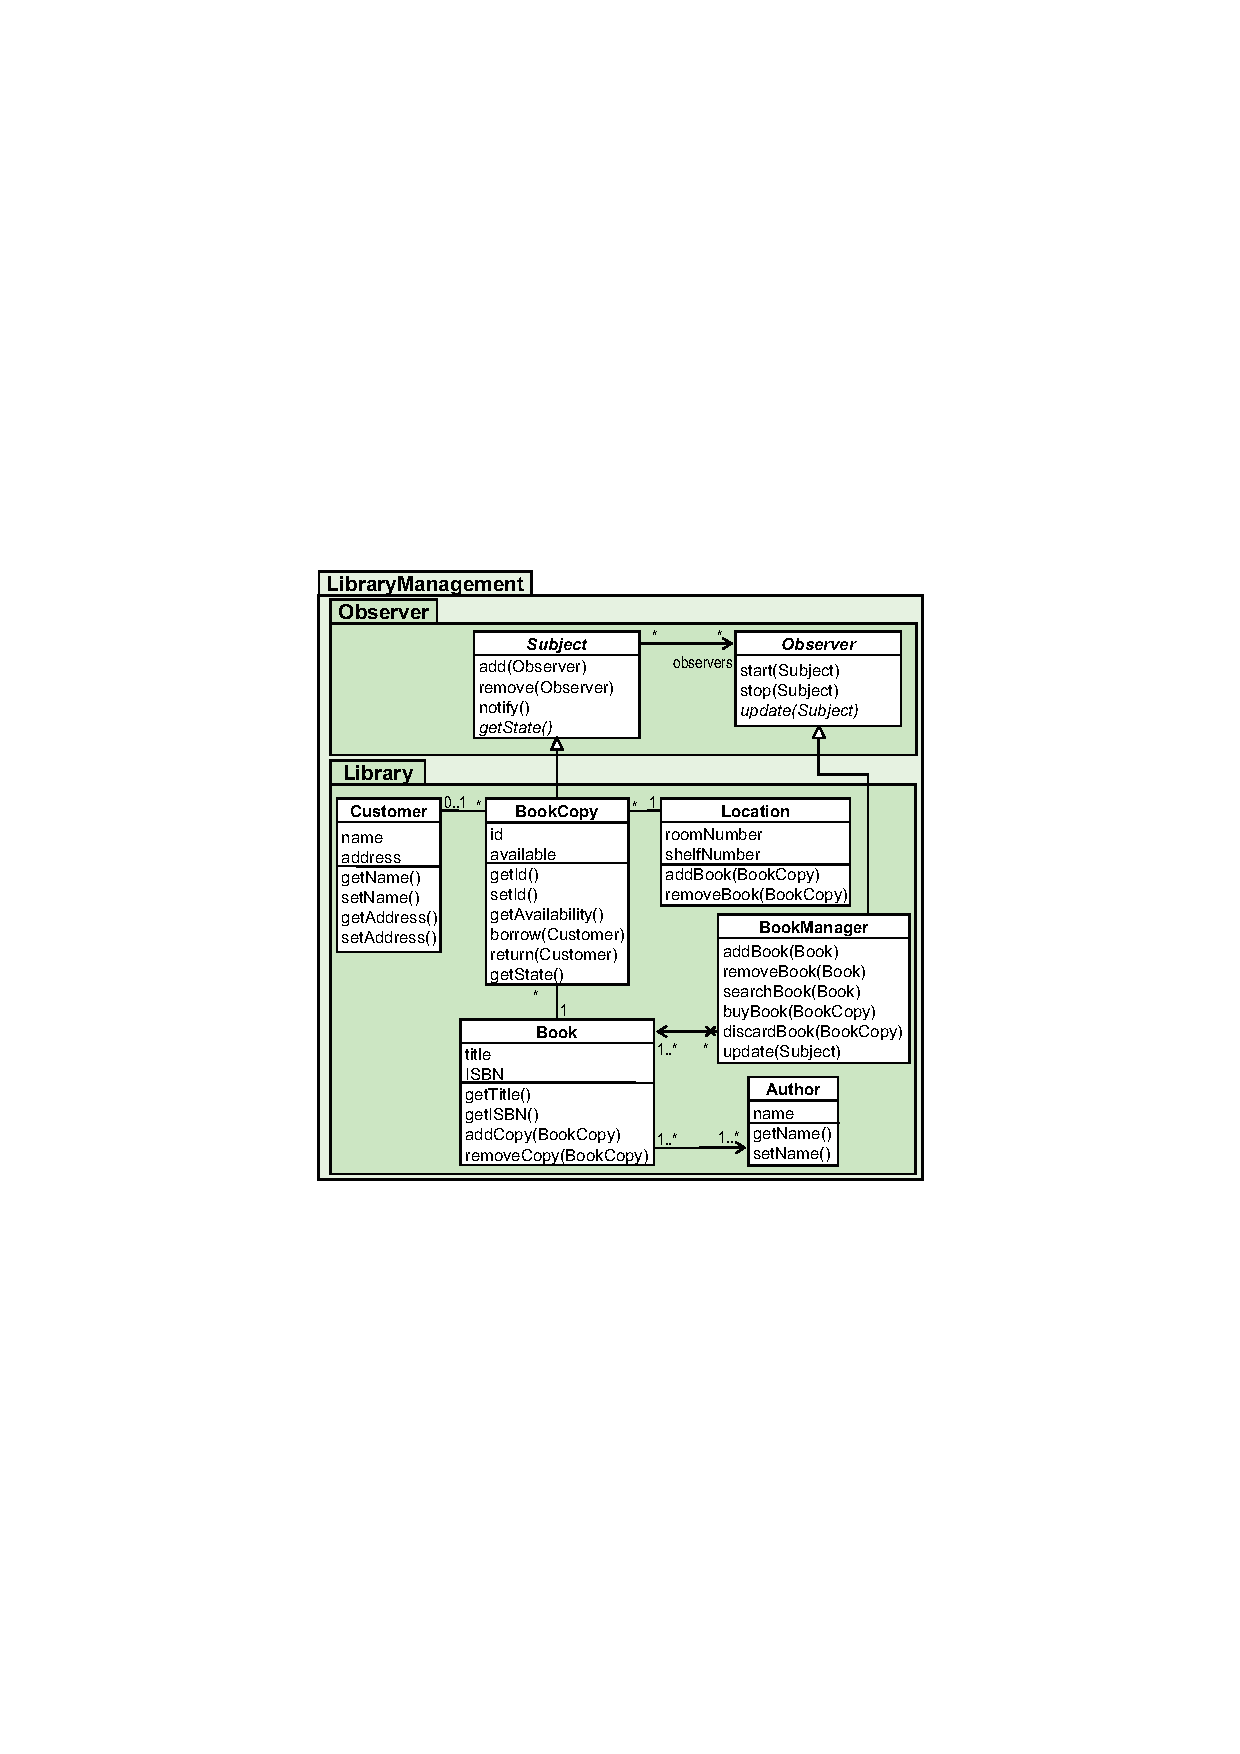
\includegraphics[width=0.4\linewidth]{figures/figure1}
	\caption{xxx (Quelle zitieren, wenn nicht selbst erstellt)}
	\label{fig:xxx}
\end{figure}

%-----------------------------------------------------------------------
\subsection{Tabellen}
%-----------------------------------------------------------------------

Jede Tabelle muss im Fließtext referenziertw werden. Für Tabellen gelten die selben Regeln, wie für Abbildungen (siehe dazu Abschnitt \ref{sec:abbildungen}).

Eine Beispiel einer Tabelle ist in Tabelle \ref{tab:xxx} zu finden:
\begin{table}
	\centering
	\begin{tabular}{| >{\bfseries}l | c | r | }
		\hline
			\rowcolor{orange} \bfseries Linksbündig & \bfseries Zentriert & \bfseries Rechtsbündig \\
		\hline
		\hline
			Zeile 1 & xxx & xxx \\\hline
			Zeile 2 & xxx & \dots \\\hline
			\multirow{2}{*}{Zeile3}
			& xxx & xxx \\\cline{2-3}
			& xxx & xxx \\\hline
		\hline
			\multicolumn{3}{| c |}{xxx} \\\hline
	\end{tabular}
	\caption{xxx (Quelle angeben)}
	\label{tab:xxx}
\end{table}

Bitte beachten Sie, dass Tabellen generell so einfach wie möglich gehalten werden sollen. Tabelle \ref{tab:xxx} dient unter anderem dazu Studierenden zu zeigen, wie Tabellen in \LaTeX\xspace erstellt werden können und wie Farben verwendet werden.
%%%%%%%%%%%%%%%%%%%%%%%%%%%%%%%%%%%%%%%%%%%%%%%%%%%%%%%%%%%%%%%%%%%%%%%%
\chapter{Konkrete Problemstellung -- Umfeldbeschreibung}
\label{sec:problemdescription}
%%%%%%%%%%%%%%%%%%%%%%%%%%%%%%%%%%%%%%%%%%%%%%%%%%%%%%%%%%%%%%%%%%%%%%%%

In diesem Kapitel wird die eigentliche Problemlösung in einem oder mehreren Unterkapiteln ausgeführt. Die Strukturierung dieser Kapitel ist naturgemäß sehr stark von der konkreten Aufgabenstellung abhängig. Der Name dieses Kapitels ist anzupassen, z.B. Umfeldbeschreibung -- Fallbeispiel \dots, konkreter schreiben je nach Art Diplomarbeit/Fragestellung.
\makeatletter\ifthesis@masterthesis
Nachfolgend einige Beispiele für unterschiedliche Arten von Diplomarbeiten.

Bei einer Software-Entwicklungsarbeit bieten sich folgende Unterkapitel an:
\begin{itemize}
	\item Im Kapitel \enquote{Design} sollte die konzeptionelle Lösung vorgestellt, diskutiert und begründet werden. Das Ergebnis dieses Kapitels könnte beispielsweise eine Protokoll-Architektur sein.
	\item Im Kapitel \enquote{Modelle} erfolgt üblicherweise das Feindesign. In diesem Kapitel könnten beispielsweise einzelne Protokolle bzw. Algorithmen aus der vorher definierten Protokoll-Architektur eingeführt und diskutiert werden. Achtung: Generell darauf achten, bei der eingangs erläuterten Notation zu bleiben und nicht Synonyme zu verwenden, verwirrt den Leser.
	\item Das Kapitel \enquote{Implementierung} sollte sich dann vorwiegend mit den Details der Umsetzung befassen. In diesem Kapitel sollte nur im Ausnahmefall exemplarisch Quellcode vorgesehen werden. Vielmehr sollten alle Probleme, die bei der Realisierung aufgetreten sind, dokumentiert, interpretiert und die Lösung erläutert werden.
\end{itemize}

Bei einer Arbeit zu einem abstrakteren Thema, bei dem ein oder mehrere Fallbeispiele aus der industriellen Praxis bearbeitet werden, bieten sich folgende Unterkapitel an:
\begin{itemize}
	\item Im Unterkapitel \enquote{Analyse der Problemstellung} wird die konkrete Problemstellung (die Situation im betrachteten Unternehmen) der Fallbeispiele beschrieben. Das Ergebnis dieses Kapitels könnte eine schematische Netzwerk- oder Applikationsarchitektur sein.
	\item Im Unterkapitel \enquote{Fallbeispiel} sollte sich (analog zur Implementierung in der Software-Entwicklung) mit den konkreten Details der Umsetzung befassen. Hier wird dargelegt, wie das zuvor identifizierte Lösungsschema konkret zur Anwendung gelangen kann bzw. welche Probleme während des Umsetzungsprojekts aufgetreten sind.
\end{itemize}

Bei einer Arbeit, deren Grundlage eine Auswahl eines Softwaresystems ist, bieten sich folgende Unterkapitel an:
\begin{itemize}
	\item IST-Analyse
	\item Hardware und Softwareausstattung
	\item Beschreibung der Geschäftsprozesse
	\item Schwachstellenanalyse des Unternehmens
	\item SOLL-Konzeption
	\item Auswahlverfahren möglicher verfügbarer Systeme -- Kriterienkatalog
	\item Einführung des neuen Systems
\end{itemize}

Bei einer Arbeit, deren Fokus auf der Durchführung und Auswertung von Fragebögen liegt, bieten sich folgende Unterkapitel an:
\begin{itemize}
	\item Im Kapitel \enquote{Problemstellung und Fragebogendesign} wird die fachliche Problemstellung detailliert erläutert und der Inhalt des Fragebogens in Bezug zur Problemstellung dargestellt.
	\item Im Kapitel \enquote{Befragungsmethode} werden die Untersuchungsobjekte (z.B. Praktische Ärzte), die Grundgesamtheit (Anzahl praktische Ärzte in Venezuela), Stichprobengesamtheit und das Verfahren zur Stichprobenziehung und das Erhebungsverfahren (Verteilung und Rücklauf der Fragebögen) beschrieben.
	\item Im Kapitel \enquote{Auswertungsmethode} werden die möglichen Auswertungsmethoden aufgelistet und ggf. begründet die ausgewählte Methode beschrieben.
	\item Im Kapitel \enquote{Befragungsdurchführung} wird die Untersuchungsdurchführung (z.B. Zeit, Ort der Befragung, Zeitraum der gesamten Befragung, besondere für das Untersuchungsergebnis oder zukünftige Forschungsarbeiten relevante Vorkommnisse etc.) dargestellt.
\end{itemize}

Hier intensive Rücksprache mit Ihren jeweiligen Fachbetreuern halten, mehrere Diplomarbeiten der Fakultät zu diesem Themenbereich durchsehen. Unabhängig vom Typ der Diplomarbeit werden im nachfolgenden Kapitel die konkreten Ergebnisse beschrieben.
\fi\makeatother
\chapter{Hinweise zur Literatur}
\label{sec:references}

\section{Literatursuche}

Der Vollzugang zu einigen Publikationen ist nur intern aus dem TU-Netz möglich. Um auf möglichst viele Papers extern zugreifen zu können, wird von der TU Wien eine \href{http://www.zid.tuwien.ac.at/tunet/vpn/extern/}{VPN-Zugangsmöglichkeit} angeboten, diesen VPN-Zugang bitte gleich einrichten.

Besonders ergiebig sind folgende Search-Engines:\\
\href{http://academic.research.microsoft.com/}{Microsoft Academic}\\
\href{http://dl.acm.org/}{ACM-Datenbank}\\
\href{http://scholar.google.com/}{Google Scholar}

Wir empfehlen, vor Beginn Ihrer Arbeit einige Diplomarbeiten, die am INSO oder generell an der Fakultät für Informatik verfaßt wurden, zu Ihrem Themenbereich zu suchen und Aufbau, Schreibstil, Art der Abbildungen etc. durchzuschauen. Arbeiten finden Sie \href{http://media.obvsg.at/tuw?query=grechenig&metaname=swishdefault&submit=Suche+starten&sbm=tuw*&lbm=*&lbc=*&searchtype=sim&.cgifields=metaname}{hier}.

Weitere Datenbanken und Suchmaschinen:\\
\href{http://rzblx1.uni-regensburg.de/ezeit/search.phtml?bibid=UBTUW&colors=7&lang=de}{Elektronische Zeitschriftenbibliothek der TU Wien}\\
\href{http://citeseer.ist.psu.edu/index;jsessionid=BF9BD5A89D42210F60E5CA88B40BAD9C}{Scientific Literature Digital Library (CiteSeer)}\\
\href{http://www.ingentaconnect.com/}{Ingenta}\\
\href{http://www.theiet.org/resources/inspec/}{INSPEC}

Journals:\\
\href{http://ieeexplore.ieee.org/}{IEEE - Institute of Electrical and Electronics Engineers, Inc. - Library}\\
\href{http://www.springerlink.com/?MUD=MP}{Verlag Springer - Springer Link}\\
\href{http://www.elsevier.com/wps/find/homepage.cws_home}{Elsevier}

Bibliotheken und Online-Kataloge:\\
\href{http://search.obvsg.at/primo_library/libweb/action/search.do?vid=ACC}{Online-Kataloge des Österreichischen Bibliothekenverbundes}\\
\href{http://aleph.ub.tuwien.ac.at/}{Online-Katalog der TU Wien} (ALEPH)\\
\href{http://www.informatik.uni-trier.de/}{Digital Bibliography \& Library Project (DBLP) of University of Trier}\\
\href{http://liinwww.ira.uka.de/bibliography/}{The Collection of Computer Science Bibliographies}

\section{BibLatex}

Biblatex beitet verschiedene Möglichkeiten an um Literatur zu referenzieren. Die beiden häufigsten Befehle sind \verb|\cite| und \verb|\citeauthor|.

Beispiele wie referenziert werden kann:\\
\citeauthor{fankhauser:2009:softwaretechnik-security} beschreiben in \cite{fankhauser:2009:softwaretechnik-security} \dots\\
In \cite{schanes:2011:voip-fuzzer} zeigt \citeauthor{schanes:2011:voip-fuzzer} wie \dots
Weitere Informationen können von \cite{oasis:2010:homepage} in \cite{oasis:2010:homepage} entnommen werden.

Wir empfehlen JabRef um die Literaturdatenbank zu verwalten.
\chapter{Algorithmen und Quellcode}

\section{Beispiele für Quellcode}

Beispiel eines Quellcodes ist im Quellcode \ref{lst:shortcode} zu finden.

\begin{lstlisting}[caption={Short code},label=lst:shortcode]
//Start Program
System.out.println("Hello World!");
//End Program
\end{lstlisting}


\section{Beispiele für Algorithmen}

Algorithmus \ref{alg:samplealgorithm} dient als Beispiel.

\begin{algorithm}[t]
\SetKwData{Left}{left}
\SetKwData{This}{this}
\SetKwData{Up}{up}
\SetKwFunction{Union}{Union}
\SetKwFunction{FindCompress}{FindCompress}
\SetKwInOut{Input}{input}
\SetKwInOut{Output}{output}

\Input{A bitmap $Im$ of size $w\times l$}
\Output{A partition of the bitmap}

\BlankLine

\emph{special treatment of the first line}\;
\For{$i\leftarrow 2$ \KwTo $l$}{
\emph{special treatment of the first element of line $i$}\;
\For{$j\leftarrow 2$ \KwTo $w$}{\label{forins}
\Left$\leftarrow$ \FindCompress{$Im[i,j-1]$}\;
\Up$\leftarrow$ \FindCompress{$Im[i-1,]$}\;
\This$\leftarrow$ \FindCompress{$Im[i,j]$}\;
\If(\tcp*[r]{O(\Left,\This)==1}){\Left compatible with \This}{\label{lt}
\lIf{\Left $<$ \This}{\Union{\Left,\This}}\;
\lElse{\Union{\This,\Left}\;}
}
\If(\tcp*[r]{O(\Up,\This)==1}){\Up compatible with \This}{\label{ut}
\lIf{\Up $<$ \This}{\Union{\Up,\This}}\;
\tcp{\This is put under \Up to keep tree as flat as possible}\label{cmt}
\lElse{\Union{\This,\Up}}\tcp*[r]{\This linked to \Up}\label{lelse}
}
}
\lForEach{element $e$ of the line $i$}{\FindCompress{p}}
}
\caption{Sample algorithm}\label{alg:samplealgorithm}
\end{algorithm}

%%%%%%%%%%%%%%%%%%%%%%%%%%%%%%%%%%%%%%%%%%%%%%%%%%%%%%%%%%%%%%%%%%%%%%%%
\chapter{Ergebnisse}
\label{sec:results}
%%%%%%%%%%%%%%%%%%%%%%%%%%%%%%%%%%%%%%%%%%%%%%%%%%%%%%%%%%%%%%%%%%%%%%%%

Die Resultate der Arbeit präsentieren und nach Möglichkeit aussagekräftige, eigenständige Abbildungen einbauen. Namen des Kapitels konkretisieren, an jeweilige Arbeit anpassen -- Lösungsvorschlag/Implementierung im Titel des Kapitels benennen.
\makeatletter\ifthesis@masterthesis
Bei einer Soft\-ware-Ent\-wicklungs\-arbeit ggf. eine Beschreibung der Qualitätsmerkmale der neuen Implementierung (Performance, Sicherheit, Messergebnisse etc.) geben.

Bei einer Arbeit zu einem abstrakteren Architekturthema können hier die Eigenschaften nach der Anwendung der konzipierten Architektur beschrieben werden. Kommt sie in mehreren Fallbeispielen zum Einsatz, erfolgt hier ein Vergleich der jeweiligen Ergebnisse (z.B. gab es Unterschiede im Umsetzungserfolg, die sich auf konkrete Eigenschaften der betrachteten Fallbeispiele zurückführen lassen).

Bei einer Arbeit zur Softwareauswahl und Einführung wird eine Beschreibung von Qualitätseigenschaften des mit der Einführung neu geschaffenen SOLL-Zustands gegeben.

Bei einer Arbeit, deren Fokus auf der Durchführung und Auswertung von Fragebögen liegt, erfolgt in diesem Kapitel die Auswertung der Fragebögen.
\fi\makeatother
\makeatletter\ifthesis@masterthesis
%%%%%%%%%%%%%%%%%%%%%%%%%%%%%%%%%%%%%%%%%%%%%%%%%%%%%%%%%%%%%%%%%%%%%%%%
\chapter{Diskussion}
\label{sec:discussion}
%%%%%%%%%%%%%%%%%%%%%%%%%%%%%%%%%%%%%%%%%%%%%%%%%%%%%%%%%%%%%%%%%%%%%%%%

Den akademischen Wert der Arbeit hervorheben, Vergleich mit verwandten Arbeiten: In welchem Verhältnis stehen die Ergebnisse der Diplomarbeit zu den Ergebnissen anderer Studien? Wo gibt es Unterschiede, wo Gemeinsamkeiten? Warum?

Diskussion offener Punkte, Darstellen der Stärken und Schwächen der vorliegenden Ergebnisse.
\fi\makeatother
%%%%%%%%%%%%%%%%%%%%%%%%%%%%%%%%%%%%%%%%%%%%%%%%%%%%%%%%%%%%%%%%%%%%%%%%
\chapter{Zusammenfassung und Ausblick}
\label{sec:conclusion}
%%%%%%%%%%%%%%%%%%%%%%%%%%%%%%%%%%%%%%%%%%%%%%%%%%%%%%%%%%%%%%%%%%%%%%%%

\makeatletter\ifthesis@masterthesis
Die Zusammenfassung ist nach der Kurzfassung der am häufigsten gelesene Teil, da viele Leser aus Zeitknappheit Arbeiten im Schnellverfahren konsumieren und rasch zur Zusammenfassung blättern. Hier hat man die Chance, dem Leser noch einmal die zentralen Ideen und Ergebnisse der Diplomarbeit zu vermitteln.

Im Gegensatz zur Kurzfassung sind die Leser mit der Problemstellung und der Terminologie bereits vertraut. In der Länge hat man deutlich mehr Spielraum als bei der Kurzfassung, die Zusammenfassung sollte inklusive Ausblick 2 bis max. 10 Seiten umfassen. Hier sollten kompakt die Antworten auf die in der Zielsetzung aufgeworfenen Fragen (Hypothesen) gegeben werden.

Neben einer Zusammenfassung der wichtigsten Ergebnisse sollte auch ein Ausblick gegeben werden: Aufzeigen des Bedarfs an zukünftiger Forschung, potentielle Anwendungsmöglichkeiten der vorgestellten Lösung etc.

In Summe sollte die Zusammenfassung dem Leser die wissenschaftliche und, wenn vorhanden, praktische Relevanz der Arbeit klar und verständlich darlegen.
\fi\makeatother

% insert bibliography and such stuff
\BackMatter

\cleardoublepage
\appendix

%%%%%%%%%%%%%%%%%%%%%%%%%%%%%%%%%%%%%%%%%%%%%%%%%%%%%%%%%%%%%%%%%%%%%%%%
\chapter{\appendixlabel}
%%%%%%%%%%%%%%%%%%%%%%%%%%%%%%%%%%%%%%%%%%%%%%%%%%%%%%%%%%%%%%%%%%%%%%%%



\end{document}
